\begin{frame}[t]{Input Modeling}{What the CO$_2$ input data contains}

  \begin{columns}[T,totalwidth=\textwidth]
    \begin{column}{0.48\textwidth}
      \textbf{Data from Electricity Map}
      \begin{itemize}
        \item 5 regions: DE, IT, SE, CN, US
        \item 201,600 samples per region
        \item 1,008,000 samples in total
        \item 5-minute time resolution
        \item Time span: 2022-01-01 to 2026-06-16
      \end{itemize}
    \end{column}
    \begin{column}{0.48\textwidth}
      \textbf{Data quality}
      \begin{itemize}
        \item Most values are measured, not estimated.
        \item Estimated-value share is below 3\% for DE, ES, FR, SE.
        \item For China all values are estimated.
        \item The dataset is usable for region-level input modeling.
      \end{itemize}
    \end{column}
  \end{columns}
\end{frame}

\begin{frame}[t]{Input Modeling}{Average grid intensity differs strongly}
  \small

  \centering
  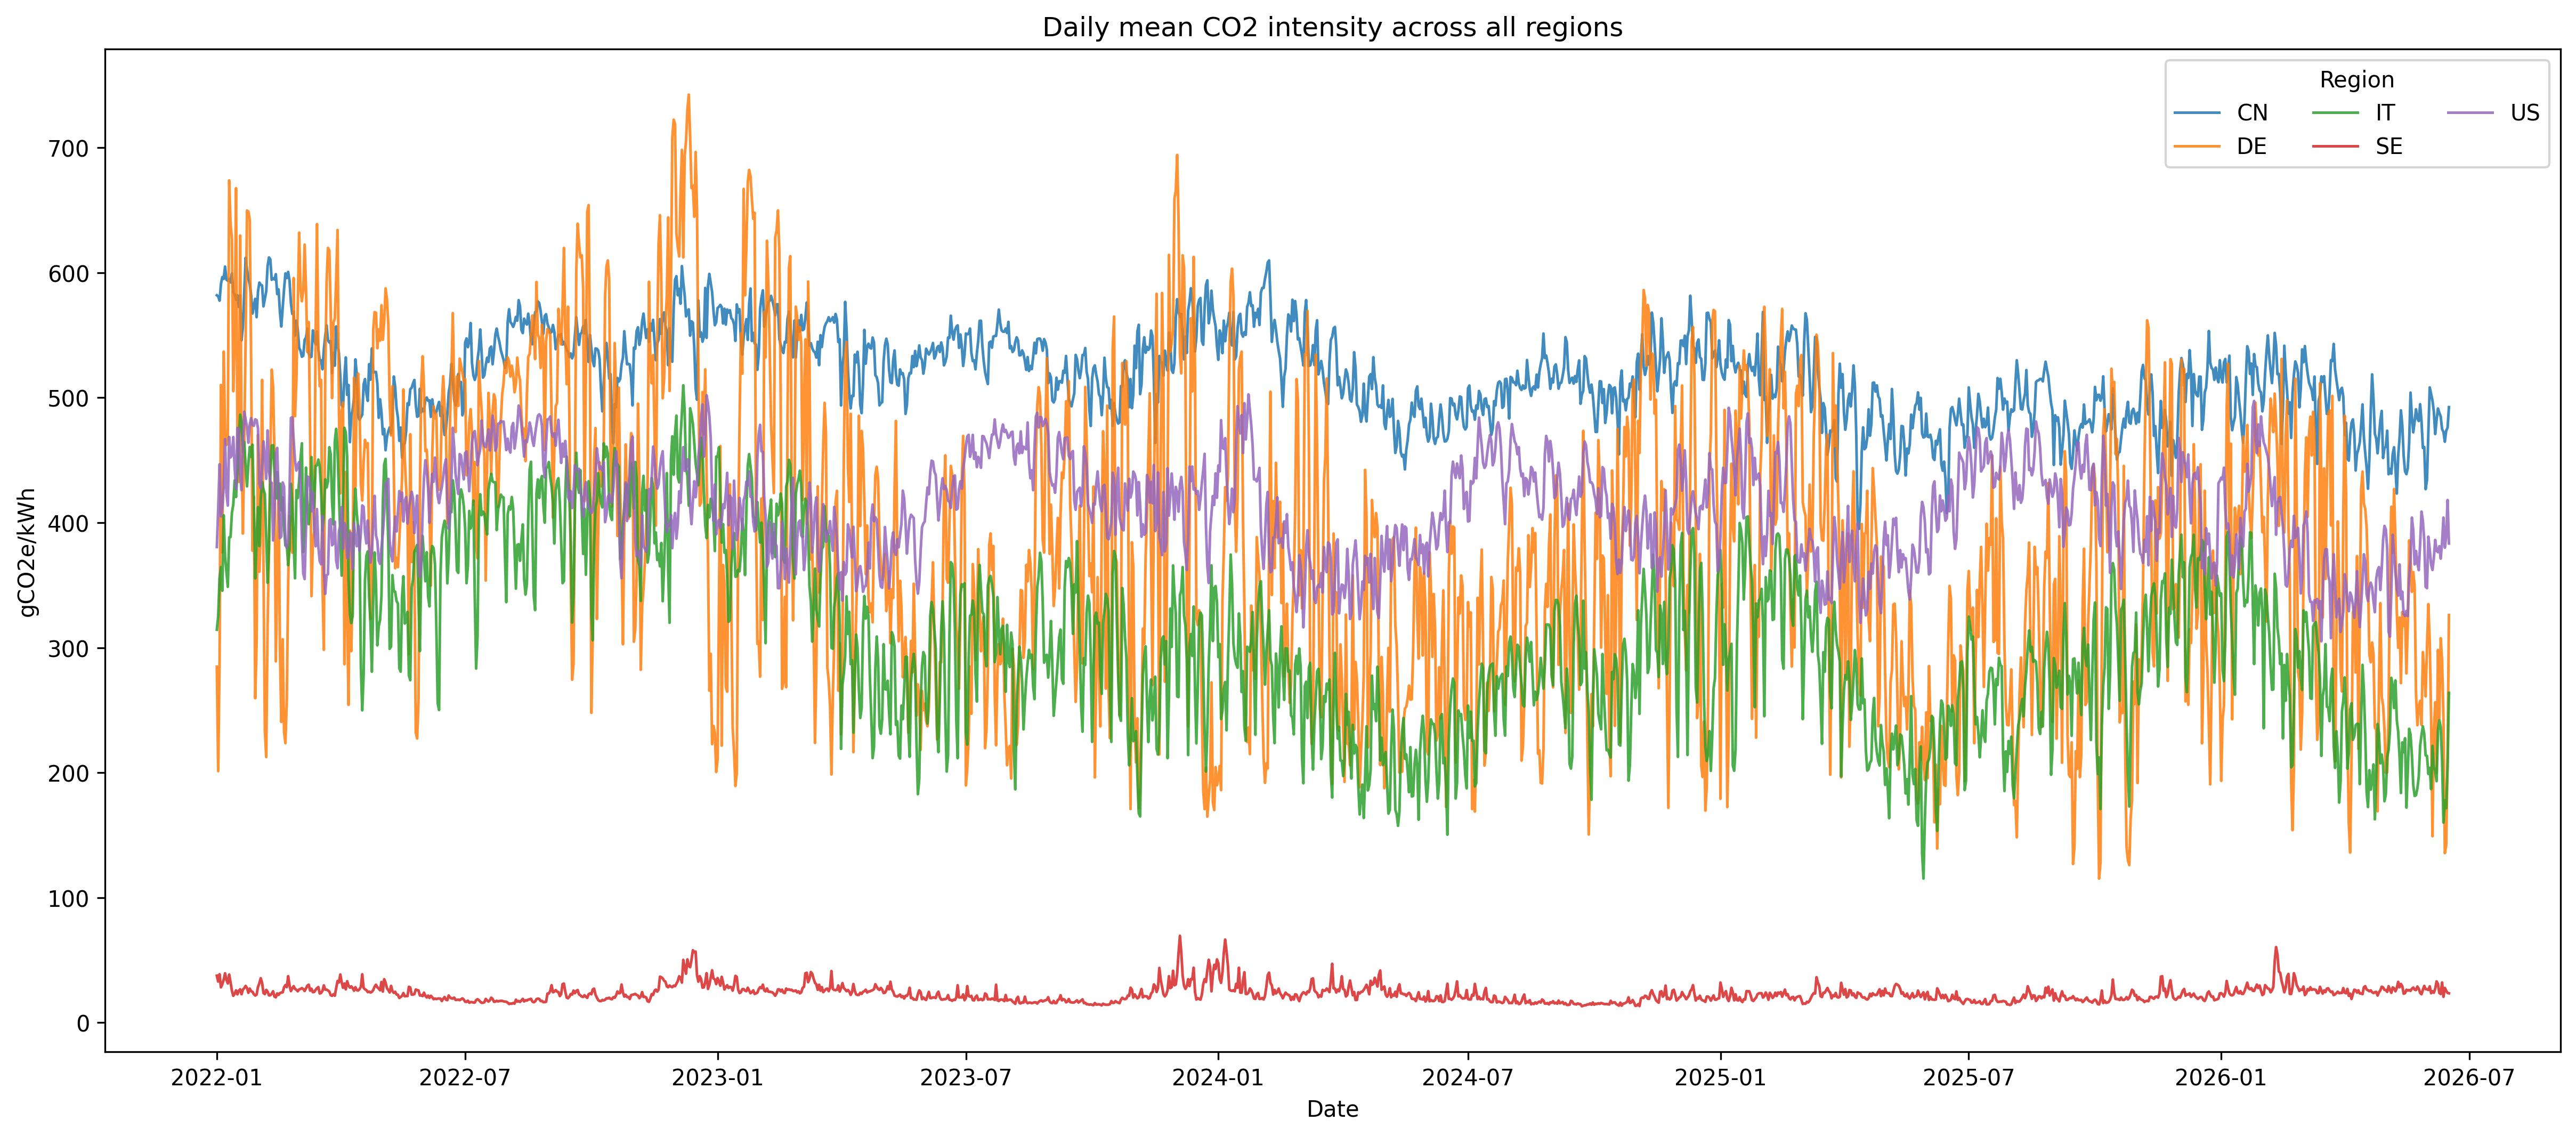
\includegraphics[width=\textwidth,height=0.66\textheight,keepaspectratio]{assets/daily_co2_intensity.png}

  \vspace{0.1cm}
  \begin{itemize}
    \item Mean intensities span from 23 to 519 gCO$_2$eq/kWh.
    \item DE is about 16.3x higher than SE on average.
  \end{itemize}
\end{frame}

\begin{frame}[t]{Input Modeling}{Absolute and relative variability tell
  different stories}
  \small

  \centering
  \resizebox{0.46\textwidth}{!}{%
    \begin{tabular}{lrrr}
\toprule
Region & Mean & Std.\ dev. & Coeff.\ of\ variation \\
\midrule
DE & 348 & 129.24 & 0.37 \\
ES & 132 & 48.66 & 0.37 \\
FR & 29 & 13.53 & 0.46 \\
IT & 280 & 72.27 & 0.26 \\
SE & 21 & 7.07 & 0.33 \\
\bottomrule
\end{tabular}
%
  }

  \vspace{0.2cm}
  \begin{itemize}
    \item DE has the largest absolute swing, so pause/resume can avoid
      high-emission windows.
    \item Region-specific thresholds are necessary because ``high carbon'' is
      not the same numeric value everywhere.
  \end{itemize}

  \vspace{0.4cm}
  \begin{block}{Main takeaway}
    The data is dense enough for simulation input modeling, but the regions are
    very different and should not share one global threshold.
  \end{block}

\end{frame}

\begin{frame}[t]{Input Modeling}{The time series is not independent}

  \centering
  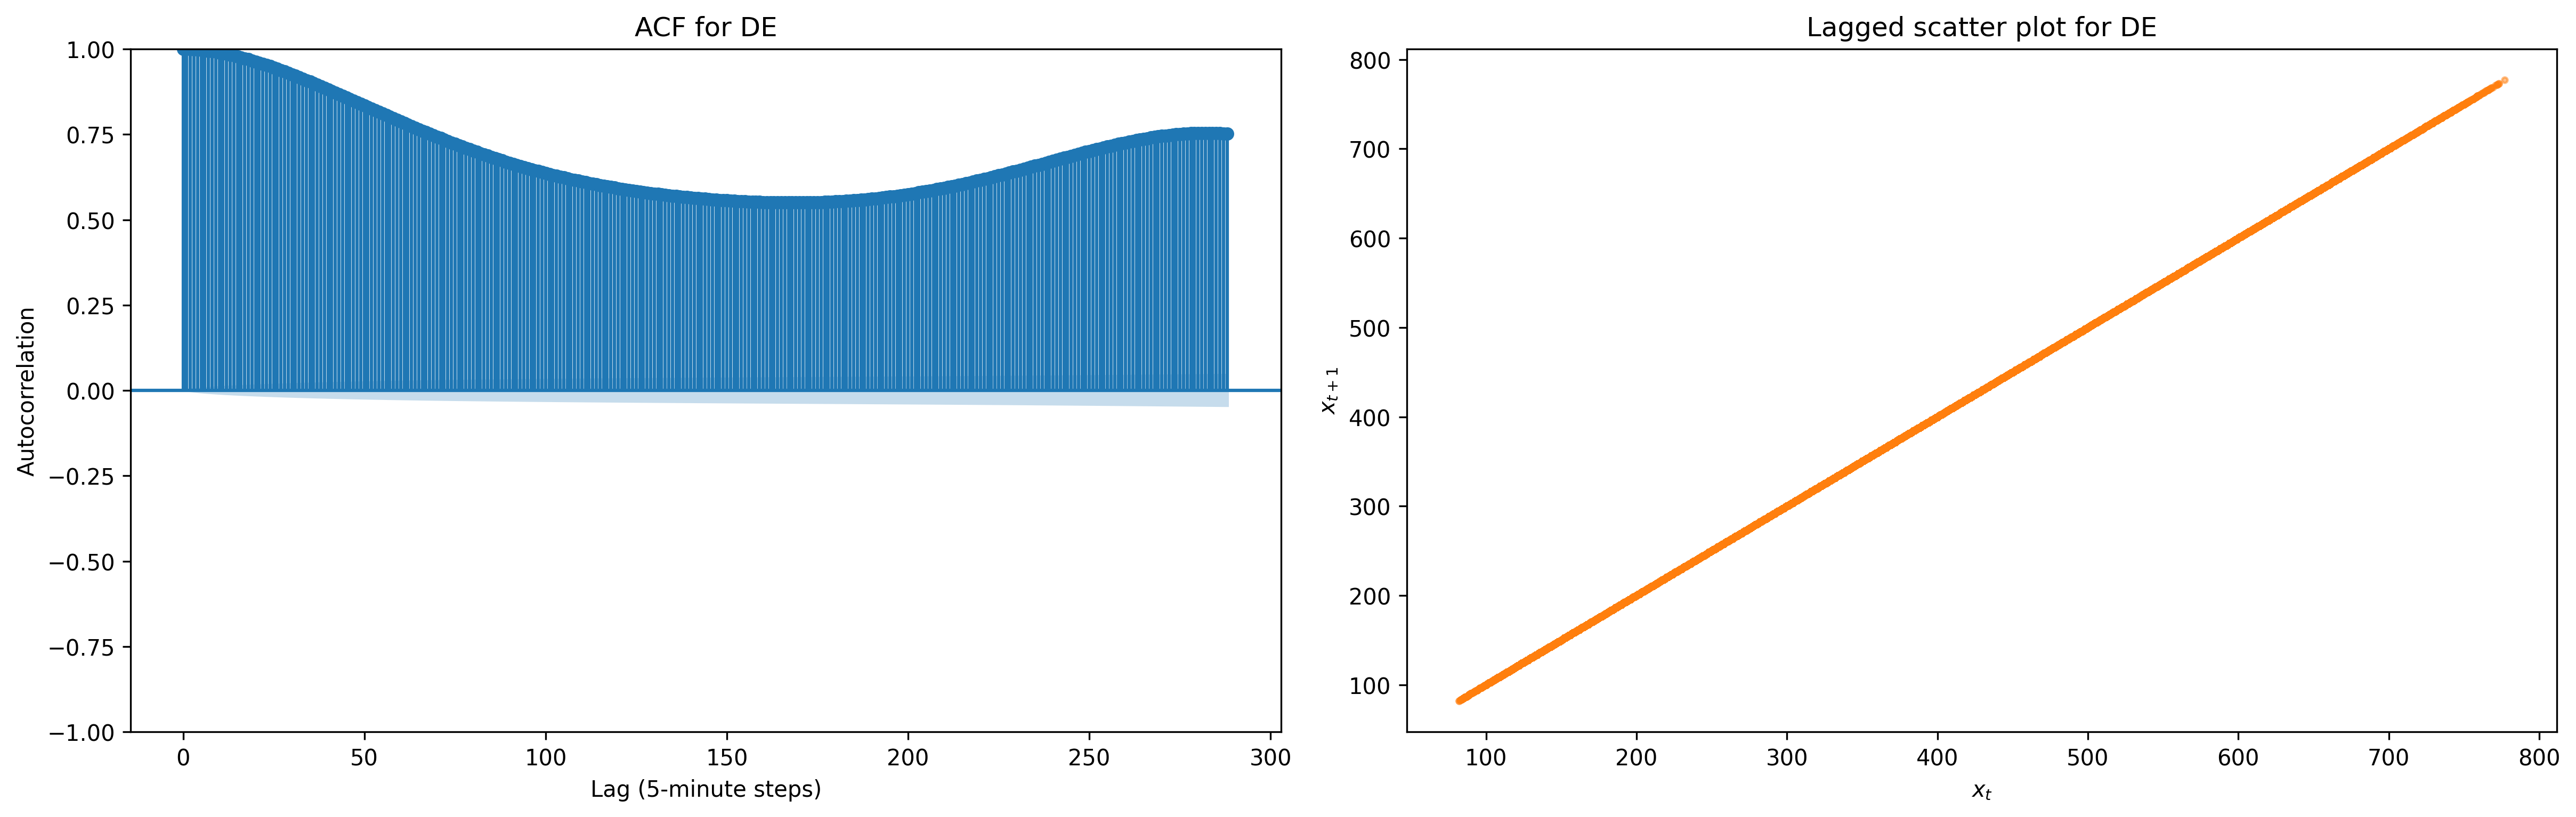
\includegraphics[width=\textwidth,height=0.58\textheight,keepaspectratio]{assets/acf_lag.png}

  \vspace{0.05cm}
  \begin{block}{Consequence for the training simulation}
    Lag-1 autocorrelation is 0.999 and the one-day lag is 0.694 for DE:
    chronological trace replay is more appropriate than IID sampling.
  \end{block}

\end{frame}

\begin{frame}[t]{Input Modeling}{Best-fitting distributions differ by region}

  \centering
  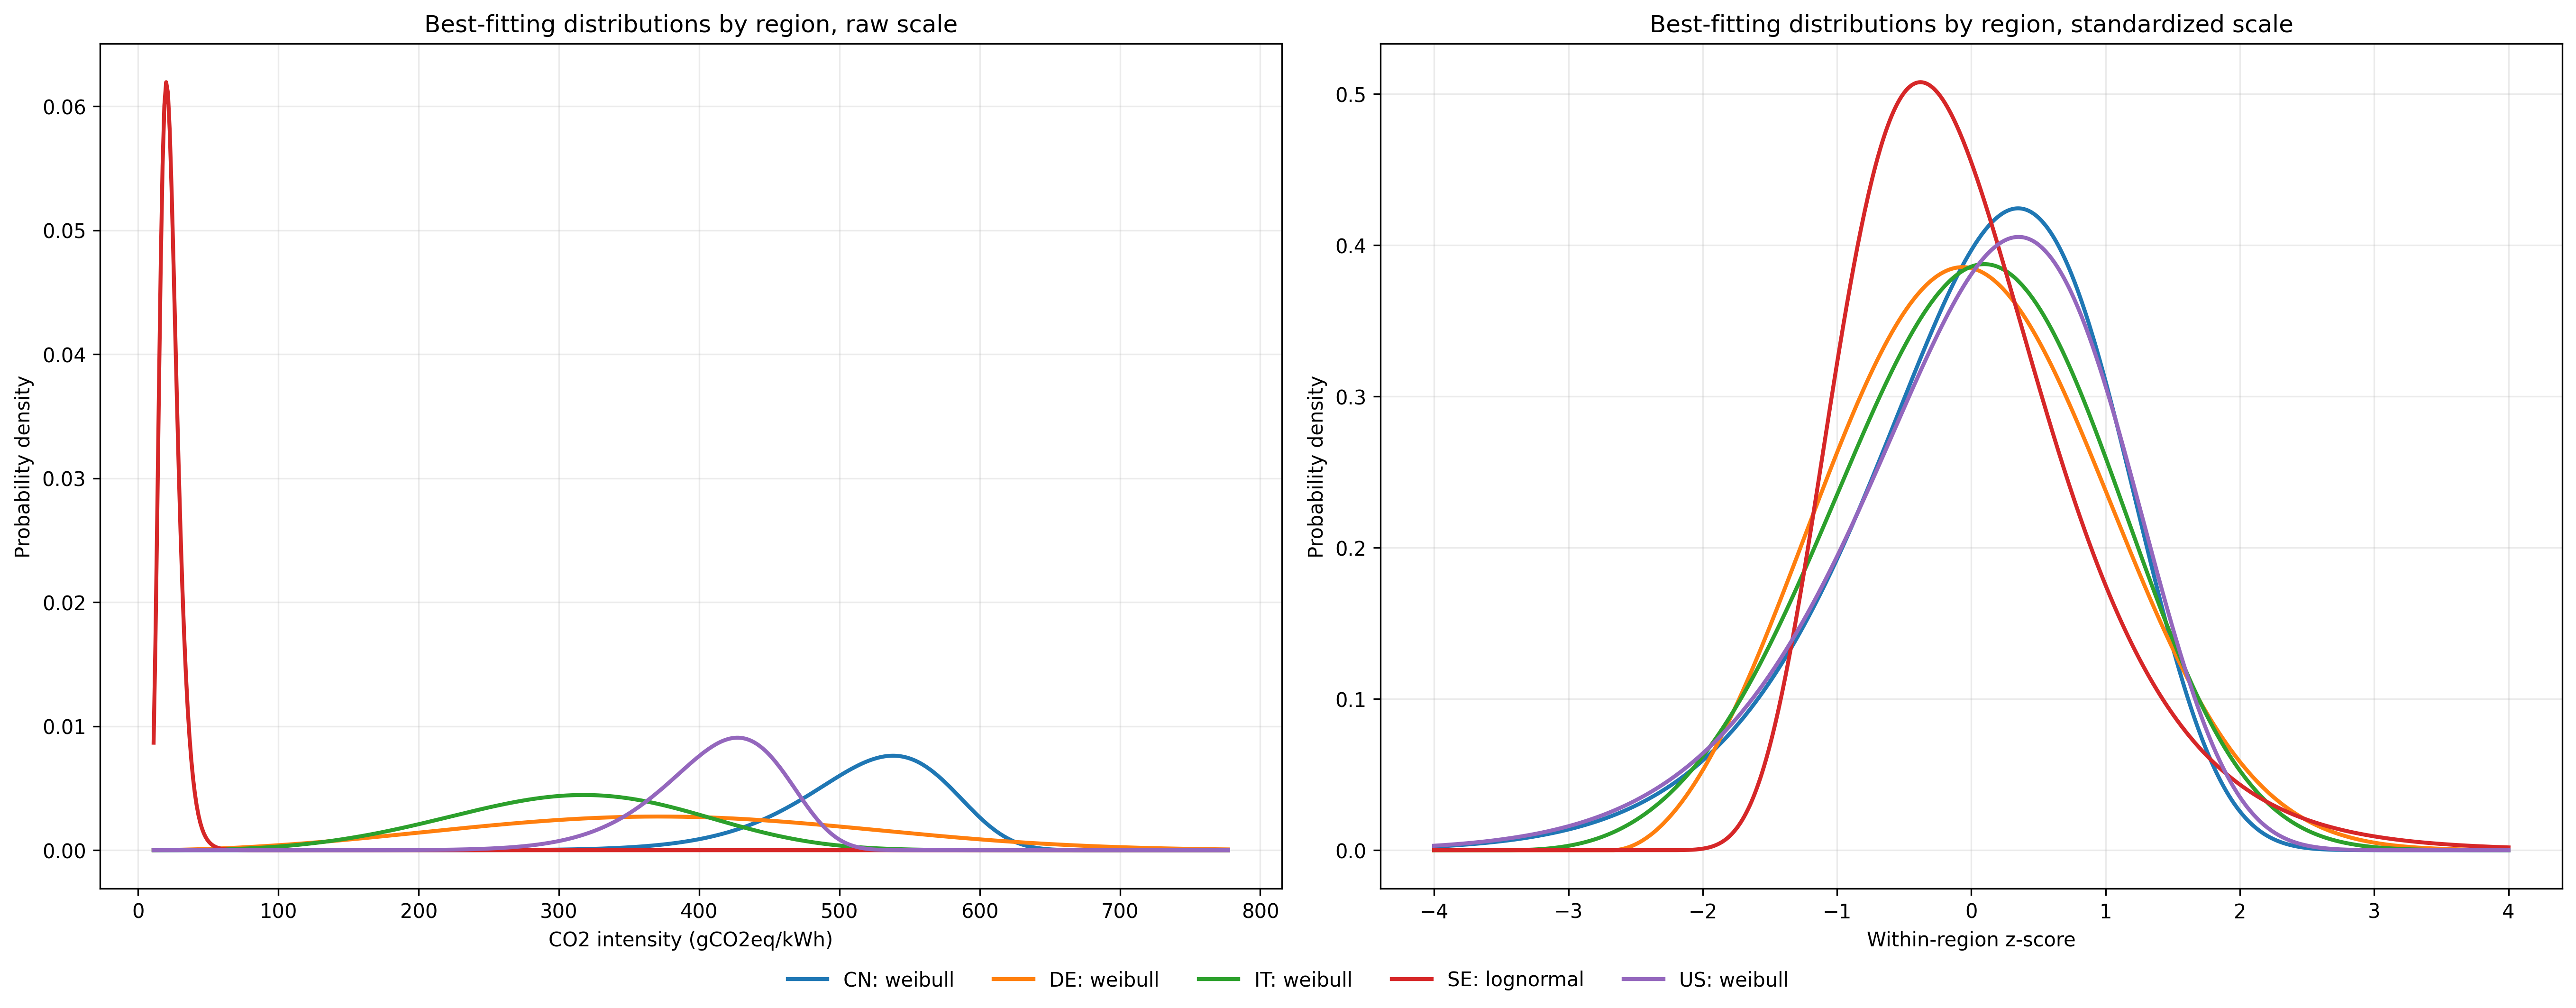
\includegraphics[width=\textwidth,height=0.68\textheight,keepaspectratio]{assets/best_fit_distributions.png}

  \vspace{0.1cm}
  \begin{itemize}
    \item SE fits Lognormal best, all others fit Weibull best.
    \item The standardized panel compares shape independent of absolute
      intensity.
  \end{itemize}

\end{frame}

\begin{frame}[t]{Input Modeling}{Q-Q and P-P diagnostics for all regions}

  \centering
  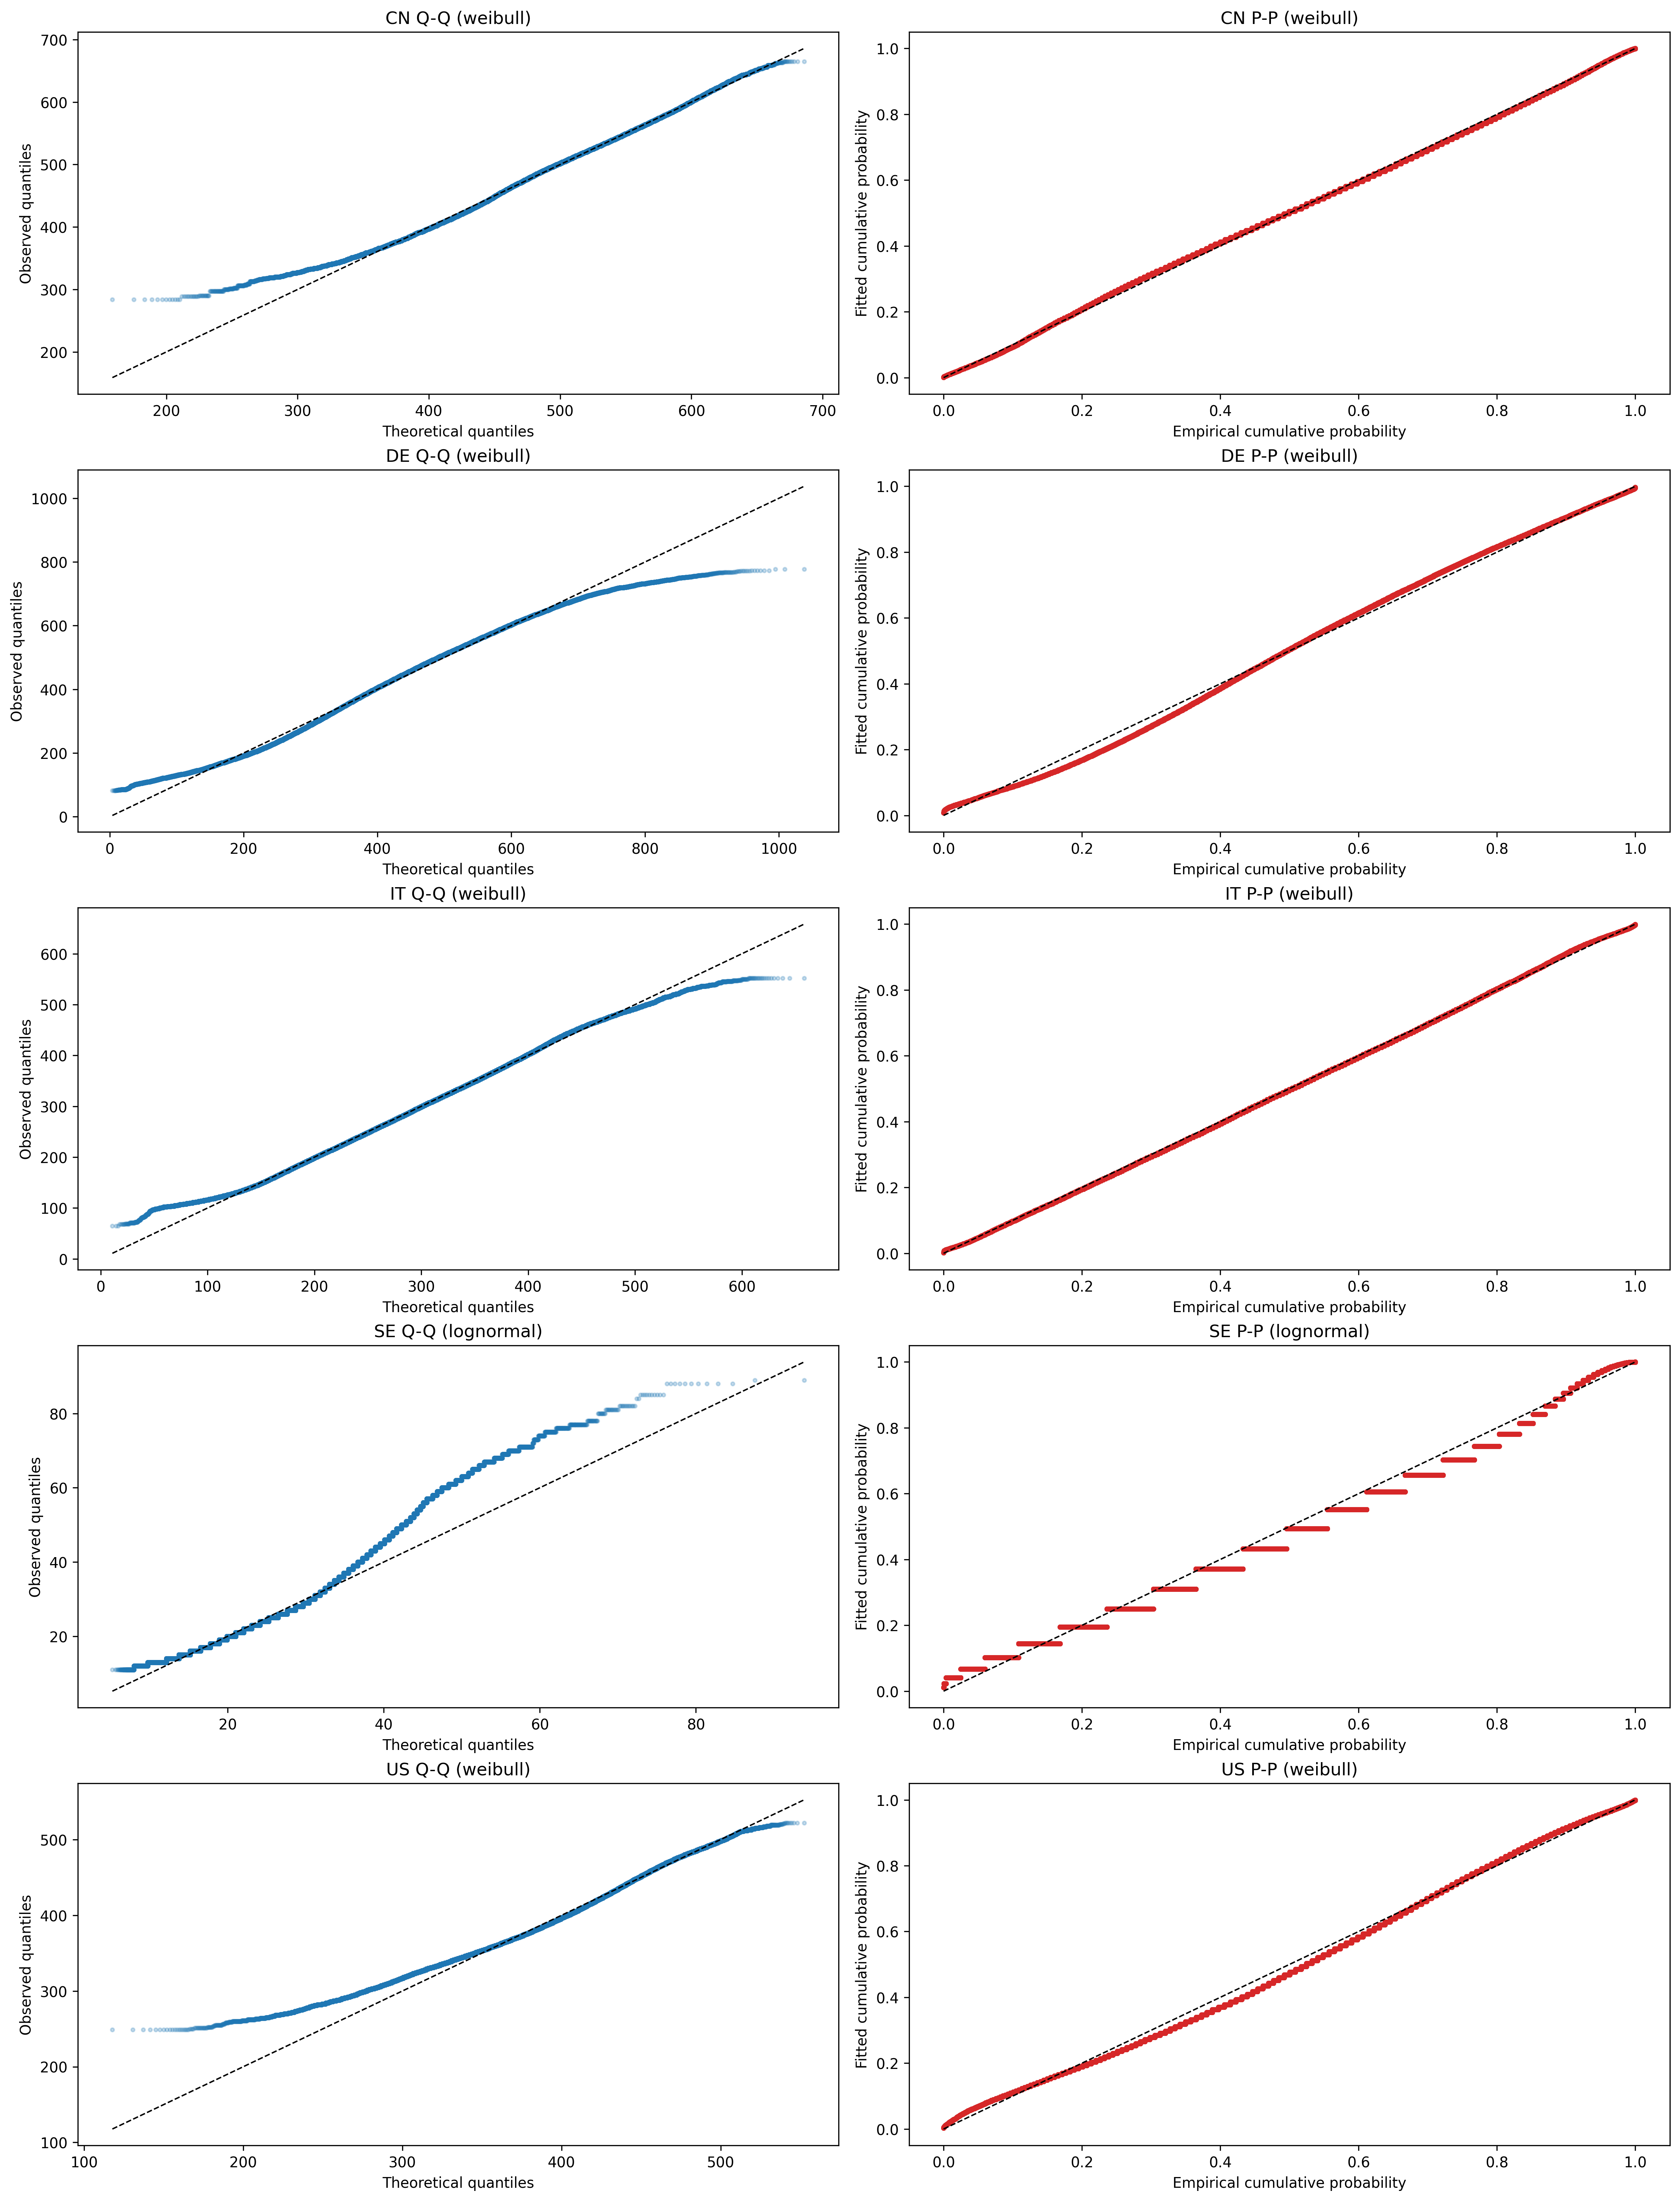
\includegraphics[width=\textwidth,height=0.76\textheight,keepaspectratio]{assets/qq_pp_plots.png}

  \vspace{0.05cm}
  \small
  Q-Q plots expose tail mismatch; P-P plots show whether the fitted CDF tracks
  the empirical CDF over the full probability range.

\end{frame}

\begin{frame}[t]{Input Modeling}{Implications for our Simulation}

  \begin{enumerate}
    \item Use historical traces for evaluation, because temporal dependence is
      strong.
    \item Calibrate pause and resume thresholds per region, not globally.
    \item Compare policies on both CO$_2$ savings and wall-clock overhead.
    \item Treat clean regions differently: low baseline emissions reduce the
      benefit of aggressive pausing.
    \item Use fitted distributions as compact input-model summaries, but keep
      trace replay as the primary validation path.
  \end{enumerate}

  \vspace{0.35cm}
  \begin{block}{Most important finding}
    Carbon-aware scheduling potential is driven by both the average grid mix
    and the temporal variability around that average.
  \end{block}

\end{frame}
